En este capítulo se dispone el análisis realizado en base a los requisitos presentados
en el capítulo 3, haciendo uso del lenguaje de modelado UML. Concretamente,
el capítulo describe:

\begin{itemize}
\item El modelo conceptual de los datos usados en la aplicación, elaborado a
partir de los requisitos de información.
\item Los casos de uso, que describen los pasos que componen los procesos habituales del proyecto.
\item El modelo de interfaz de usuario, en el que se presenta un prototipo de la
navegación y de las interfaces.
\end{itemize}

%%%%%%%%%%%%%%%%%%%%%%%%%%%%%%%%%%%%%%%%%%%%%%%%%%%%%%
%%%%%%%%%%%%%%%%%%%%%%%%%%%%%%%%%%%%%%%%%%%%%%%%%%%%%%

\section{Modelo conceptual}

De acuerdo a lo reflejado en el apartado 3.2.2 se presenta el diagrama~\ref{fig:modelo-conceptual}  en el
que se identifican los principales tipos de datos, sus atributos y las relaciones entre
ellos.

A continuación se detallan cada uno de los tipos de datos reflejados en el modelo
conceptual.

\begin{figure}[htbp]
    \centering
    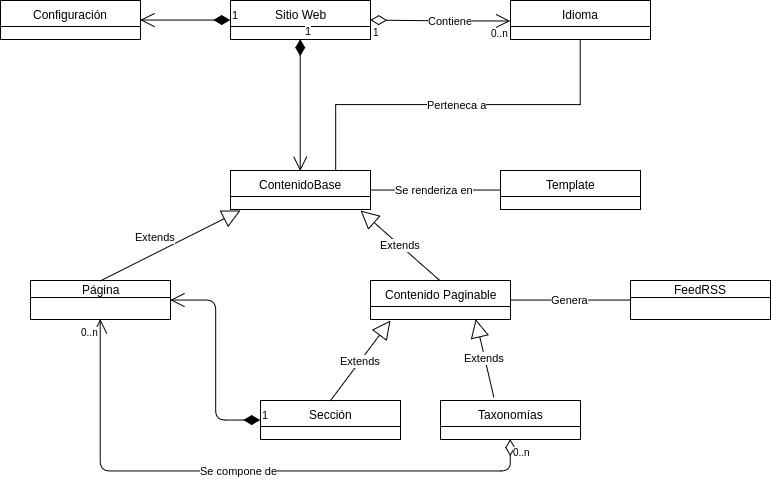
\includegraphics[width=1.1\textwidth]{4_analisis/modelo_conceptual}
    \caption{Modelo conceptual}
    \label{fig:modelo_conceptual}
\end{figure}

\subsection{Sitio web}

Represetan el sitio web generado a partir de todos los contenidos que lo componen.

Relaciones:
\begin{itemize}
    \item Esta compuesto por varios contenidos.
    \item Está compuesto por una configuración.
\end{itemize}

\subsection{Configuración}

Represetan la configuración básica del sitio.

Relaciones:
\begin{itemize}
    \item Pertence a un sitio web.
\end{itemize}

\subsection{Idioma}

Representa a los idiomas disponibles en sitio.

Relaciones:
\begin{itemize}
    \item Pertence a un sitio web.
\end{itemize}

\subsection{Contenido base}

Representa cualquier contenido que existe en un sitio.

Relaciones:
\begin{itemize}
    \item Pertenece a un sitio web.
    \item Se relaciona con una template en la que se tiene que renderizar.
    \item Se relaciona con un idioma.
\end{itemize}

\subsection{Contenido paginable}

Representa a un contenido, que a su vez está compuesto por otros contenidos, lo que implica
que es paginable.

Relaciones:
\begin{itemize}
    \item Extiende un contenido base.
\end{itemize}

\subsection{Página}

Representa la página que redacta un usuario.

Relaciones:
\begin{itemize}
    \item Extiende un contenido base.
    \item Pertenece a una sección.
    \item Se clasifica en varias taxonomías.
\end{itemize}

\subsection{Sección}

Representa a un conjunto de contenidos.

Relaciones:
\begin{itemize}
    \item Está compuesto por varias páginas.
    \item Extiende un contenido base.
\end{itemize}

\subsection{Taxonomías}

Representa la clasificacion de contenidos.

Relaciones:
\begin{itemize}
    \item Extiende un contenido base.
    \item Contiene varias páginas.
\end{itemize}

\subsection{Template}

Representa la template HTML en la que se renderiza un contenido

Relaciones:
\begin{itemize}
    \item Se relaciona con un contenido.
\end{itemize}

\subsection{Feed RSS}

Representa la representación RSS de un contendo paginable

Relaciones:
\begin{itemize}
    \item Pertence a un contenido paginable.
\end{itemize}

%%%%%%%%%%%%%%%%%%%%%%%%%%%%%%%%%%%%%%%%%%%%%%%%%%%%%%
%%%%%%%%%%%%%%%%%%%%%%%%%%%%%%%%%%%%%%%%%%%%%%%%%%%%%%

\section{Modelo de casos de uso}

El modelo de casos de uso representa las interacciones entre los actores y el siste-
ma, desarrollado a partir de los requisitos descritos anteriormente.

\subsubsection{Caso de uso: configuración del sitio}

\subsubsection{Caso de uso: creación de contenidos}

\subsubsection{Caso de uso: clasificación de contenidos}

\subsubsection{Caso de uso: internacionalicación}

\subsubsection{Caso de uso: definición de taxonomías}

\subsubsection{Caso de uso: definición de plantillas}

\subsubsection{Caso de uso: generación del sitio}


%%%%%%%%%%%%%%%%%%%%%%%%%%%%%%%%%%%%%%%%%%%%%%%%%%%%%%
%%%%%%%%%%%%%%%%%%%%%%%%%%%%%%%%%%%%%%%%%%%%%%%%%%%%%%

\section{Modelo de interfaz de usuario}
